% !TeX root = ../main.tex

\begingroup
\raggedbottom
\section{本章例题集}

\begin{workedexample}[由幅度谱和相位谱恢复信号]
  \label{ex:ctft-recover-from-magnitude-phase}
  已知
  \[
    |X(\iu\omega)|=
    \begin{cases}
      1,&|\omega|<2,\\
      0,&|\omega|>2,
    \end{cases}
    \qquad
    \theta(\omega)=-2\omega
    \quad(|\omega|<2).
  \]
  求 $x(t)$。题设采用展开相位，频谱见\cref{fig:ex-ctft-phase-given}。

  \begin{figure}[H]
    \centering
    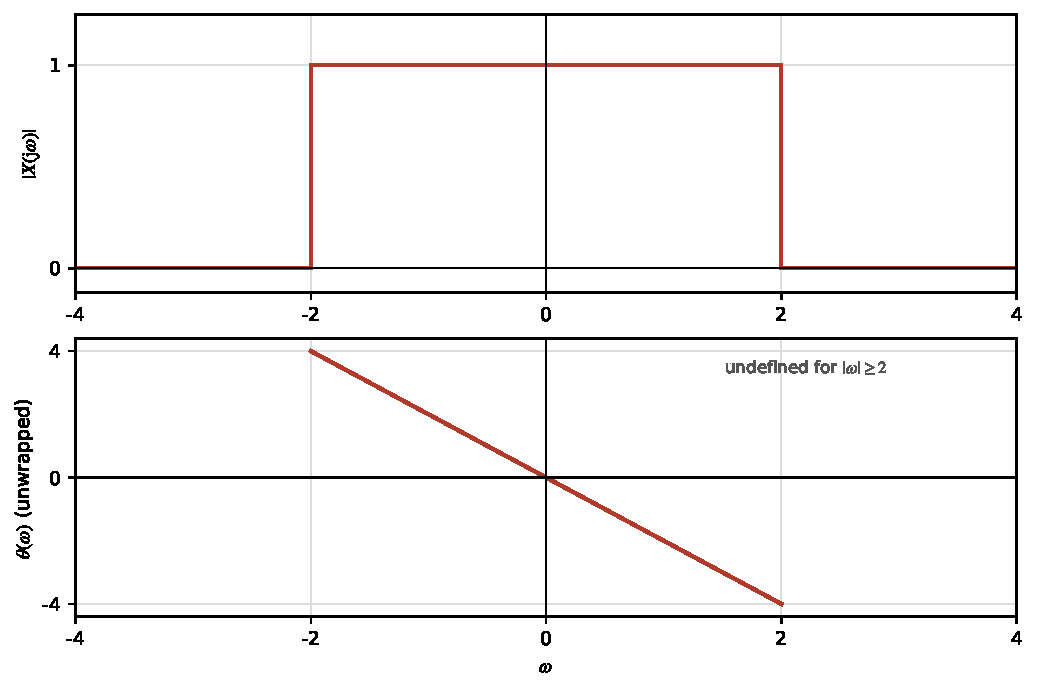
\includegraphics[width=0.76\textwidth]{06-ctft/examples/phase-recovery-given.pdf}
    \caption{例题 \ref{ex:ctft-recover-from-magnitude-phase} 的幅度谱和相位谱。}
    \label{fig:ex-ctft-phase-given}
  \end{figure}
\end{workedexample}

\begin{solution}
  由幅度和相位，
  \[
    X(\iu\omega)=\mathbf 1_{|\omega|<2}\e^{-2\iu\omega}.
  \]
  基本变换对给出
  \[
    \frac{\sin(2t)}{\pi t}
    \fourierpair
    \mathbf 1_{|\omega|<2}.
  \]
  频域中的 $\e^{-2\iu\omega}$ 对应时域延迟 $2$，所以
  \begin{equation}
    x(t)=\frac{\sin\bigl(2(t-2)\bigr)}{\pi(t-2)}.
    \label{eq:ex-ctft-phase-recovery-answer}
  \end{equation}
  直接反演也可\blue{核对延迟的符号}。$t\ne2$ 时，
  \[
    x(t)=\frac1{2\pi}\int_{-2}^{2}\e^{\iu\omega(t-2)}\dd\omega
      =\frac{\e^{2\iu(t-2)}-\e^{-2\iu(t-2)}}{2\pi\iu(t-2)}
      =\frac{\sin(2(t-2))}{\pi(t-2)}.
  \]
  $t=2$ 时直接积分得 $4/(2\pi)=2/\pi$，与极限一致。结果见\cref{fig:ex-ctft-phase-answer}。

  \begin{figure}[H]
    \centering
    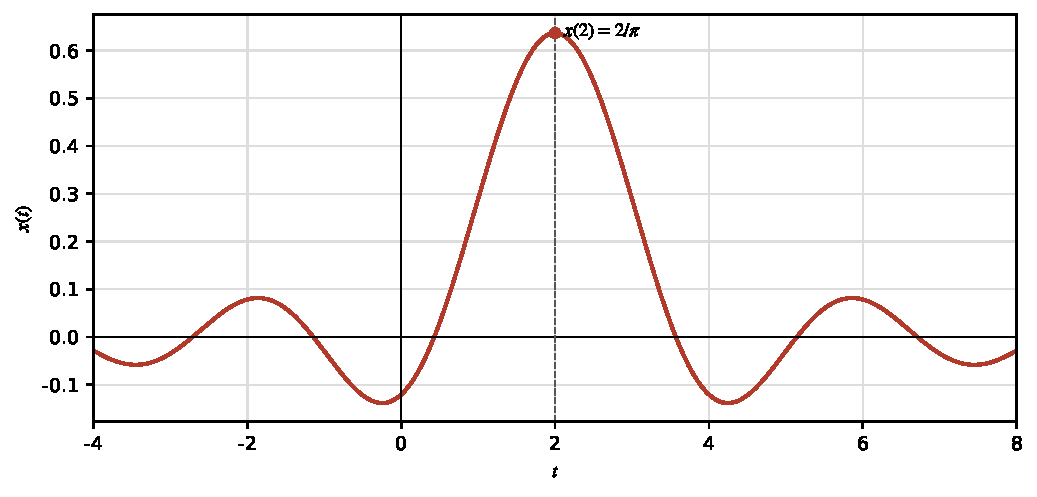
\includegraphics[width=0.72\textwidth]{06-ctft/examples/phase-recovery-answer.pdf}
    \caption{例题 \ref{ex:ctft-recover-from-magnitude-phase} 恢复出的时域信号。}
    \label{fig:ex-ctft-phase-answer}
  \end{figure}
\end{solution}

\begin{technique}
  \hl{先把幅度和相位合成复频谱}，再识别基本变换对。线性相位 $-\omega t_0$ \red{对应延迟} $t_0$；\red{只看幅度谱无法确定信号的位置}。
  若通带改为 $|\omega|<1$，相位改为 $-\omega$，同样的方法给出
  $x(t)=\sin(t-1)/[\pi(t-1)]$。
\end{technique}

\begin{workedexample}[两个移位三角脉冲之差]
  \label{ex:ctft-shifted-triangle-difference}
  定义
  \[
    \Lambda(t)=
    \begin{cases}
      1-|t|,&|t|\leq1,\\
      0,&|t|>1.
    \end{cases}
  \]
  求信号 $x(t)=\Lambda(t-3)-\Lambda(t+3)$ 的傅里叶变换。波形见\cref{fig:ex-ctft-triangle-difference-given}。
  \begin{figure}[H]
    \centering
    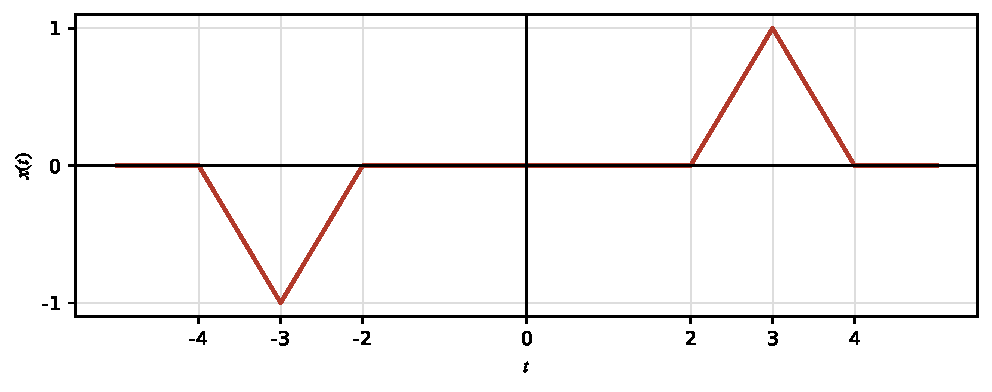
\includegraphics[width=0.72\textwidth]{06-ctft/examples/triangle-difference-given.pdf}
    \caption{例题 \ref{ex:ctft-shifted-triangle-difference} 的时域波形。}
    \label{fig:ex-ctft-triangle-difference-given}
  \end{figure}
\end{workedexample}

\begin{solution}
  单位三角脉冲可写成两个单位矩形的卷积，因此
  \[
    \Lambda(t)\fourierpair\Sa^2\left(\frac{\omega}{2}\right).
  \]
  分别应用时移性质：
  \begin{align*}
    X(\iu\omega)
    &=\Sa^2\left(\frac{\omega}{2}\right)\e^{-\iu3\omega}
      -\Sa^2\left(\frac{\omega}{2}\right)\e^{\iu3\omega}\\
    &=-2\iu\Sa^2\left(\frac{\omega}{2}\right)\sin(3\omega).
  \end{align*}
  该结果为\red{纯虚奇函数}，与 $x(t)$ 是实奇信号相符。虚部见\cref{fig:ex-ctft-triangle-difference-answer}。
  \begin{figure}[H]
    \centering
    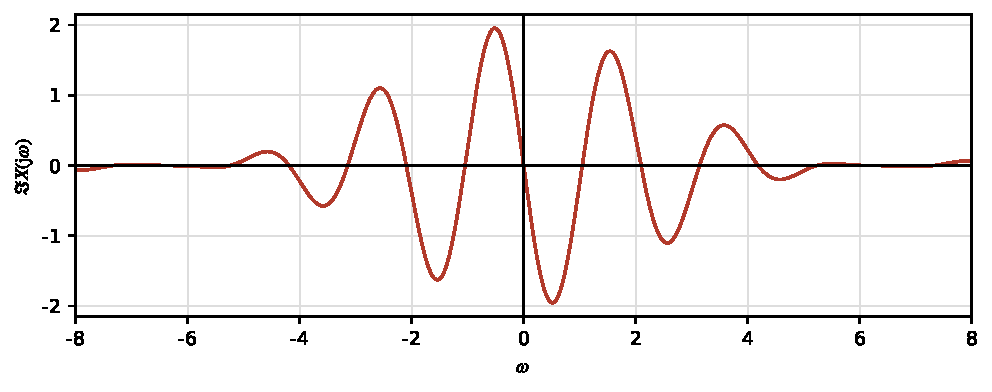
\includegraphics[width=0.72\textwidth]{06-ctft/examples/triangle-difference-answer.pdf}
    \caption{例题 \ref{ex:ctft-shifted-triangle-difference} 的虚部频谱。}
    \label{fig:ex-ctft-triangle-difference-answer}
  \end{figure}
\end{solution}

\begin{technique}
  移位信号的线性组合宜\hl{先保留指数形式}，最后再用欧拉公式合并。算完后\blue{检查时域与频域的奇偶性}，可迅速发现\red{移位符号写反}的问题。
\end{technique}

\begin{workedexample}[由频谱乘积识别三角脉冲]
  \label{ex:ctft-inverse-squared-sine}
  求
  \[
    X(\iu\omega)=\frac{2\sin^2(3\omega)}{\omega^2}
  \]
  的逆傅里叶变换。
\end{workedexample}

\begin{solution}
  令 $r(t)=\mathbf 1_{|t|<3}$，则
  \[
    r(t)\fourierpair\frac{2\sin(3\omega)}{\omega}.
  \]
  将频谱拆成两个矩形的变换：
  \[
    X(\iu\omega)
    =\frac{2\sin(3\omega)}{\omega}\,
       \frac{\sin(3\omega)}{\omega}.
  \]
  第二个因子对应 $r(t)/2$。保持 $r(\tau)$ 不动，$(r/2)(t-\tau)$ 的支撑是 $[t-3,t+3]$，重叠部分的乘积为 $1\times(1/2)$：
  \[
    \begin{array}{c|c|c}
      t\text{ 的范围}&\text{重叠区间}&x(t)\\ \hline
      -6\le t\le0&[-3,t+3]&
        \displaystyle\int_{-3}^{t+3}\frac12\dd\tau=3+\frac t2\\
      0<t\le6&[t-3,3]&
        \displaystyle\int_{t-3}^{3}\frac12\dd\tau=3-\frac t2
    \end{array}
  \]
  $|t|>6$ 时两区间错开。合并后得到三角脉冲：
  \[
    x(t)=
    \begin{cases}
      3-\dfrac{|t|}{2},&|t|\leq6,\\
      0,&|t|>6.
    \end{cases}
  \]
  峰值为 $3$，支撑为 $[-6,6]$，见\cref{fig:ex-ctft-squared-sine-answer}。
  \begin{figure}[H]
    \centering
    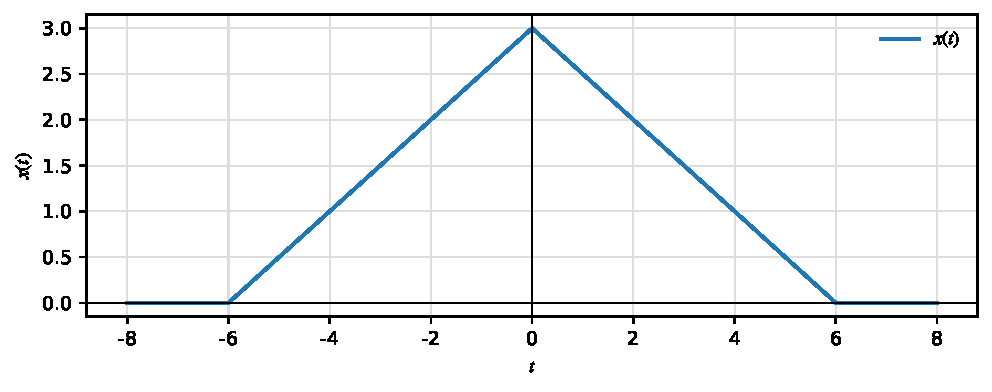
\includegraphics[width=0.72\textwidth]{06-ctft/examples/squared-sine-answer.pdf}
    \caption{例题 \ref{ex:ctft-inverse-squared-sine} 恢复出的三角脉冲。}
    \label{fig:ex-ctft-squared-sine-answer}
  \end{figure}
\end{solution}

\begin{technique}
  看到频谱中出现平方，先尝试把它\hl{拆成两个已知频谱的乘积}。\red{逆变换随后变成时域卷积}；矩形与矩形卷积\hl{可直接用重叠长度求出}。
\end{technique}

\begin{workedexample}[由输入和输出反求频率响应]
  \label{ex:ctft-recover-frequency-response}
  某连续时间 LTI 系统的输入为
  \[
    x(t)=\mathbf 1_{0<t<2},
  \]
  输出为
  \[
    y(t)=
    \begin{cases}
      t,&0\leq t\leq1,\\
      2-t,&1<t\leq2,\\
      0,&\text{其他}.
    \end{cases}
  \]
  求系统的频率响应 $H(\iu\omega)$，并写出单位冲激响应的逆变换表达式。输入和输出见\cref{fig:ex-ctft-lti-identification-given}。
  \begin{figure}[H]
    \centering
    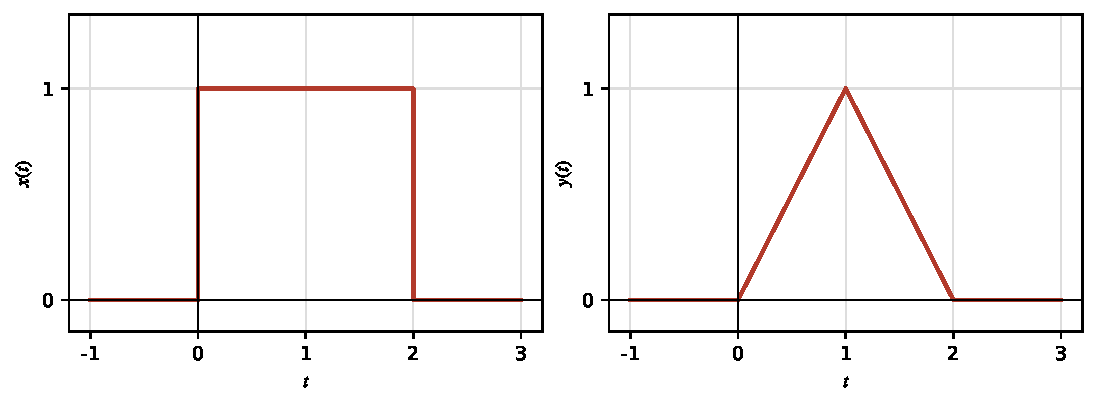
\includegraphics[width=0.86\textwidth]{06-ctft/examples/lti-identification-given.pdf}
    \caption{例题 \ref{ex:ctft-recover-frequency-response} 的输入矩形与输出三角脉冲。}
    \label{fig:ex-ctft-lti-identification-given}
  \end{figure}
\end{workedexample}

\begin{solution}
  输入是宽度为 $2$、中心位于 $1$ 的矩形：
  \[
    X(\iu\omega)=2\Sa(\omega)\e^{-\iu\omega}.
  \]
  输出等于两个 $\mathbf 1_{0<t<1}$ 的卷积。由于
  \[
    \mathbf 1_{0<t<1}
    \fourierpair
    \Sa\left(\frac{\omega}{2}\right)\e^{-\iu\omega/2},
  \]
  故
  \[
    Y(\iu\omega)=\Sa^2\left(\frac{\omega}{2}\right)\e^{-\iu\omega}.
  \]
  在 $X(\iu\omega)\ne0$ 处，
  \begin{equation}
    H(\iu\omega)
    =\frac{\Sa^2(\omega/2)}{2\Sa(\omega)}
    =\frac{\tan(\omega/2)}{\omega}.
    \label{eq:ex-ctft-recovered-frequency-response}
  \end{equation}
  上式在奇数倍 $\pi$ 处有极点。若按主值和广义函数意义解释这些极点，则形式上的逆变换为
  \[
    h(t)=\frac{1}{2\pi}\int_{-\infty}^{\infty}
    \frac{\tan(\omega/2)}{\omega}\e^{\iu\omega t}\dd\omega,
  \]
  其中积分也取相应的主值。$\tan(\omega/2)/\omega$ 为实偶函数；将复指数拆成 $\cos(\omega t)+\iu\sin(\omega t)$ 后，正弦部分为奇函数，在对称主值下积分为零，故也可写成
  \[
    h(t)=\frac1{2\pi}\operatorname{pv}\int_{-\infty}^{\infty}
      \frac{\tan(\omega/2)}{\omega}\cos(\omega t)\dd\omega.
  \]
  这个 $H$ 只是由给定输入输出得到的形式频率响应；它含有奇数倍 $\pi$ 处的极点，不能据此把 $h(t)$ 当作普通函数，也\red{不能据此断言系统因果}或 BIBO 稳定。频谱在孤立点上的取值不影响通常的逆变换；若\blue{输入频谱在一段区间内恒为零}，则那一频段的 $H$ 不能由这组输入输出确定。
\end{solution}

\begin{technique}
  先分别求 $X$、$Y$，\hl{再在输入频谱非零的频率上计算} $H=Y/X$。\blue{约分后还要检查零点}：孤立零点可能对应可去间断点或极点，整段为零则表示\red{该频带没有受到激励}。
\end{technique}

% 来源：materials/chapter3.pdf，第 23--26 页。
\begin{workedexample}[用频域乘积计算指数信号的卷积]
  \label{ex:ctft-exponential-convolution}
  设 $a,b>0$，求
  \[
    y(t)=\e^{-at}\stepfun(t)\conv\e^{-bt}\stepfun(t).
  \]
  分别讨论 $a\ne b$ 与 $a=b$。
\end{workedexample}

\begin{solution}
  由卷积性质，
  \[
    Y(\iu\omega)=\frac{1}{(a+\iu\omega)(b+\iu\omega)}.
  \]
  当 $a\ne b$ 时，令 $s=\iu\omega$ 作代数简记，设
  \[
    \frac1{(a+s)(b+s)}=\frac{A}{a+s}+\frac{B}{b+s}.
  \]
  两边乘以分母，得到 $1=A(b+s)+B(a+s)$。代入各因子的零点：
  \[
    s=-a:\quad1=A(b-a),\quad A=\frac1{b-a};
    \qquad
    s=-b:\quad1=B(a-b),\quad B=-\frac1{b-a}.
  \]
  代回，
  \[
    Y(\iu\omega)=\frac{1}{b-a}
      \left(\frac{1}{a+\iu\omega}-\frac{1}{b+\iu\omega}\right),
  \]
  逐项逆变换得到
  \[
    y(t)=\frac{\e^{-at}-\e^{-bt}}{b-a}\stepfun(t).
  \]
  当 $a=b$ 时，$Y(\iu\omega)=1/(a+\iu\omega)^2$，由\cref{eq:ctft-ramp-exponential-pair}，
  \[
    y(t)=t\e^{-at}\stepfun(t).
  \]
  两个结果在 $b\to a$ 时相接。与时域计算所得结果一致，输出在 $t<0$ 时均为零；典型波形见\cref{fig:ex-ctft-exponential-convolution}。
  \begin{figure}[H]
    \centering
    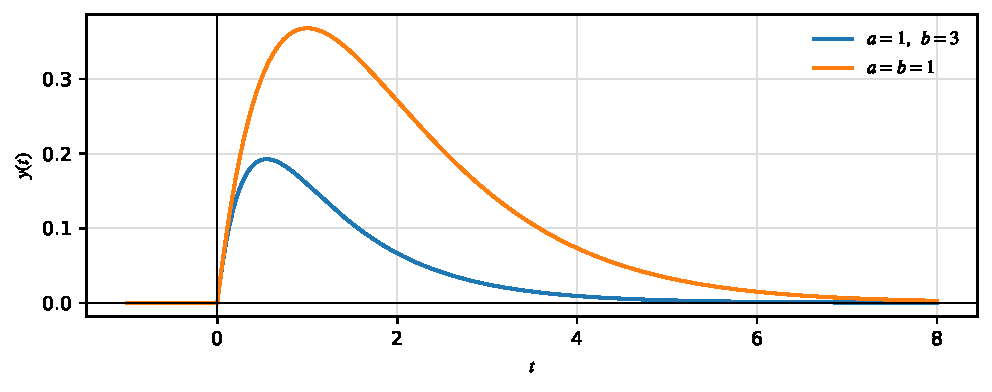
\includegraphics[width=0.72\textwidth]{06-ctft/examples/exponential-convolution-answer.pdf}
    \caption{例题 \ref{ex:ctft-exponential-convolution} 的输出：两个不同衰减率与两个相同衰减率的情形。}
    \label{fig:ex-ctft-exponential-convolution}
  \end{figure}
\end{solution}

\begin{technique}
  指数信号的卷积可\hl{先变成有理频谱的乘积}。不同的一次因子用部分分式展开；\red{相同因子合并成高次分母}，再识别 $t^n\e^{-at}\stepfun(t)$。
\end{technique}

\begin{workedexample}[由指数输入和输出求单位冲激响应]
  \label{ex:ctft-exponential-system-identification}
  某连续时间 LTI 系统在输入
  \[
    x(t)=\e^{-2t}\stepfun(t)
  \]
  作用下，输出为
  \[
    y(t)=\frac12\bigl(\e^{-t}-\e^{-3t}\bigr)\stepfun(t).
  \]
  求 $h(t)$。
\end{workedexample}

\begin{solution}
  分别变换输入和输出：
  \[
    X(\iu\omega)=\frac{1}{2+\iu\omega},\qquad
    Y(\iu\omega)=\frac12\left(\frac{1}{1+\iu\omega}
       -\frac{1}{3+\iu\omega}\right)
      =\frac{1}{(1+\iu\omega)(3+\iu\omega)}.
  \]
  $X$ \blue{在实频率轴上没有零点}，故
  \[
    H(\iu\omega)=\frac{2+\iu\omega}{(1+\iu\omega)(3+\iu\omega)}.
  \]
  令 $s=\iu\omega$，设 $H=A/(s+1)+B/(s+3)$。通分后，
  \[
    s+2=A(s+3)+B(s+1).
  \]
  代入 $s=-1$ 得 $1=2A$；代入 $s=-3$ 得 $-1=-2B$，所以 $A=B=1/2$。所求响应为
  \[
    h(t)=\frac12\bigl(\e^{-t}+\e^{-3t}\bigr)\stepfun(t),
  \]
  如\cref{fig:ex-ctft-exponential-identification}。$h(t)$ 为因果且绝对可积的函数，\red{该系统因而因果且 BIBO 稳定}。
  \begin{figure}[H]
    \centering
    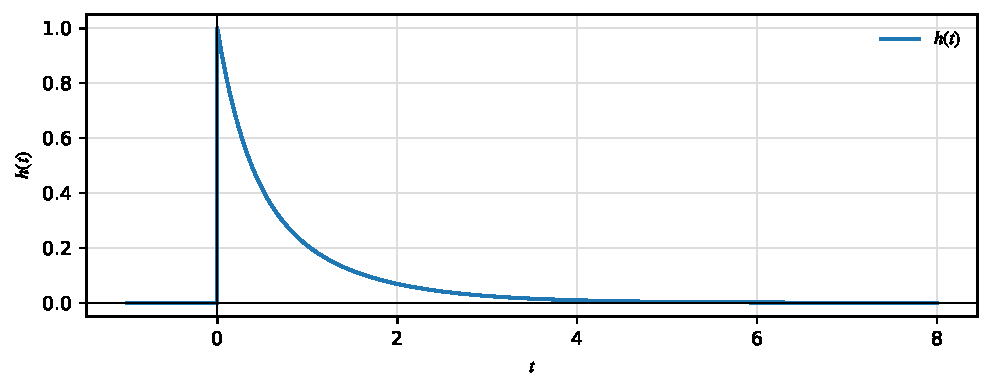
\includegraphics[width=0.70\textwidth]{06-ctft/examples/exponential-identification-answer.pdf}
    \caption{例题 \ref{ex:ctft-exponential-system-identification} 的单位冲激响应。}
    \label{fig:ex-ctft-exponential-identification}
  \end{figure}
\end{solution}

\begin{technique}
  \hl{先将输出频谱通分}，再计算 $H=Y/X$，往往比直接对多个分式作除法更简洁。求出 $h$ 后，可\blue{用支撑区间和绝对可积性检查}系统性质。
\end{technique}

\begin{workedexample}[三个一次因子的部分分式展开]
  \label{ex:ctft-three-pole-inverse}
  求
  \[
    X(\iu\omega)=\frac{1}{(1+\iu\omega)(2+\iu\omega)(3+\iu\omega)}
  \]
  的逆傅里叶变换。
\end{workedexample}

\begin{solution}
  令 $s=\iu\omega$，只将 $s$ 用作代数简记，设
  \[
    \frac{1}{(s+1)(s+2)(s+3)}
       =\frac{A}{s+1}+\frac{B}{s+2}+\frac{C}{s+3}.
  \]
  两边乘以分母后，
  \[
    1=A(s+2)(s+3)+B(s+1)(s+3)+C(s+1)(s+2).
  \]
  分别代入各因子的零点：
  \[
    \begin{array}{c|c|c}
      s&\text{剩余方程}&\text{系数}\\ \hline
      -1&1=A\times1\times2&A=1/2\\
      -2&1=B\times(-1)\times1&B=-1\\
      -3&1=C\times(-2)\times(-1)&C=1/2
    \end{array}
  \]
  逐项逆变换，
  \[
    x(t)=\left(\frac12\e^{-t}-\e^{-2t}
                      +\frac12\e^{-3t}\right)\stepfun(t)
      =\frac12\e^{-t}(1-\e^{-t})^2\stepfun(t).
  \]
  后一种写法说明 $x(t)\geq0$，且 $x(0)=0$。波形见\cref{fig:ex-ctft-three-pole-inverse}。
  \begin{figure}[H]
    \centering
    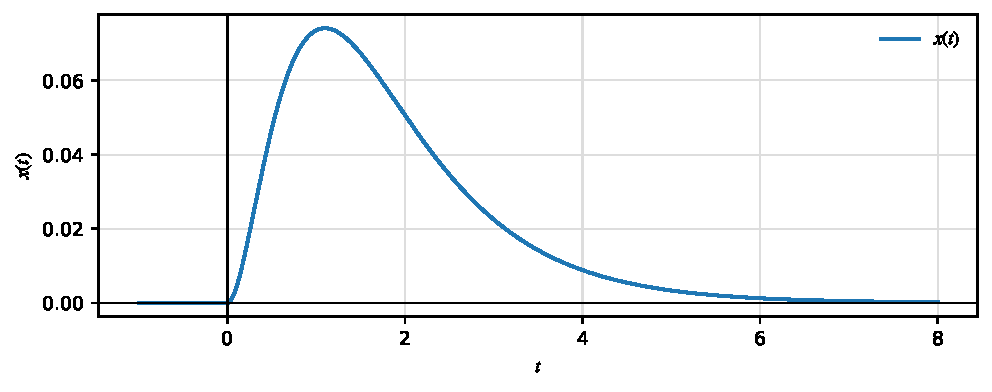
\includegraphics[width=0.70\textwidth]{06-ctft/examples/three-pole-answer.pdf}
    \caption{例题 \ref{ex:ctft-three-pole-inverse} 的时域信号。}
    \label{fig:ex-ctft-three-pole-inverse}
  \end{figure}
\end{solution}

\begin{technique}
  \blue{一次因子互异时}，\hl{通分后代入各因子的零点}即可求出系数。带正负号的指数之和\red{可再适当因式分解}，用于检查初值和符号。
\end{technique}

\begin{workedexample}[用傅里叶变换求微分方程的零状态响应]
  \label{ex:ctft-differential-equation-response}
  某因果 LTI 系统满足
  \[
    \frac{\dd^2y(t)}{\dd t^2}+4\frac{\dd y(t)}{\dd t}+3y(t)
    =\frac{\dd x(t)}{\dd t}+2x(t).
  \]
  系统初始松弛。输入为 $x(t)=\e^{-t}\stepfun(t)$，求输出 $y(t)$。
\end{workedexample}

\begin{solution}
  用时域微分性质对方程两边作变换。阶跃带来的冲激项由广义导数统一处理，得到
  \[
    [(\iu\omega)^2+4\iu\omega+3]Y(\iu\omega)
      =(\iu\omega+2)X(\iu\omega).
  \]
  代入 $X(\iu\omega)=1/(1+\iu\omega)$，有
  \[
    Y(\iu\omega)=
    \frac{\iu\omega+2}{(1+\iu\omega)^2(3+\iu\omega)}.
  \]
  分母含重根。令 $s=\iu\omega$，展开时保留 $s+1$ 的一次项和二次项：
  \[
    \frac{s+2}{(s+1)^2(s+3)}
     =\frac{A}{s+1}+\frac{B}{(s+1)^2}+\frac{C}{s+3}.
  \]
  通分后，
  \[
    s+2=A(s+1)(s+3)+B(s+3)+C(s+1)^2.
  \]
  依次代入：
  \[
    \begin{array}{c|c|c}
      s&\text{剩余方程}&\text{系数}\\ \hline
      -1&1=2B&B=1/2\\
      -3&-1=4C&C=-1/4\\
      0&2=3A+3B+C&3A=2-3/2+1/4,\quad A=1/4
    \end{array}
  \]
  因此
  \[
    Y(\iu\omega)=\frac{1/4}{1+\iu\omega}
      +\frac{1/2}{(1+\iu\omega)^2}
      -\frac{1/4}{3+\iu\omega}.
  \]
  逐项逆变换，
  \[
    y(t)=\left(\frac14\e^{-t}+\frac12t\e^{-t}
                         -\frac14\e^{-3t}\right)\stepfun(t).
  \]
  如\cref{fig:ex-ctft-differential-equation-response}，输出从零开始。虽然系统初始松弛，但\red{输入在零时刻跳变}，$\dd x/\dd t$ 含有冲激，因此不应另行强加 $y'(0^+)=0$。
  \begin{figure}[H]
    \centering
    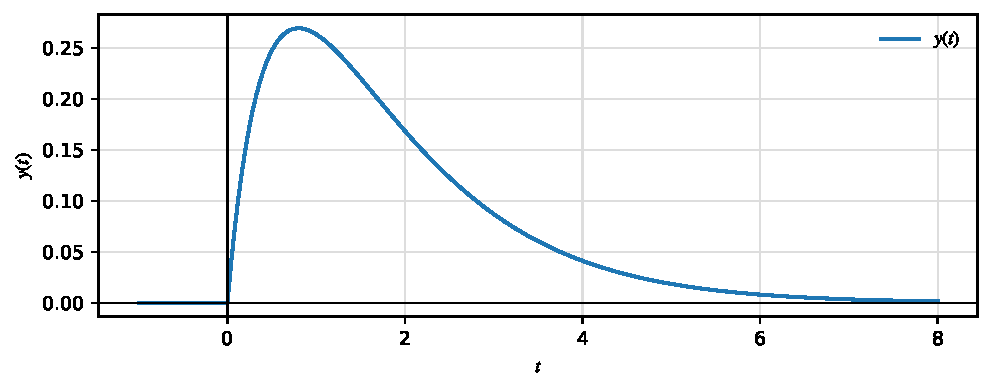
\includegraphics[width=0.70\textwidth]{06-ctft/examples/differential-equation-answer.pdf}
    \caption{例题 \ref{ex:ctft-differential-equation-response} 的零状态输出。}
    \label{fig:ex-ctft-differential-equation-response}
  \end{figure}
\end{solution}

\begin{technique}
  对初始松弛系统，\hl{先将求导转换为频域}乘以 $\iu\omega$，求出 $H$ 后再乘输入频谱。重根处的部分分式必须\red{包含从一次到最高次的所有分母项}；\blue{初值条件应区分跳变前与跳变后}。
\end{technique}

\begin{workedexample}[由两个移位三角频谱恢复信号]
  \label{ex:ctft-two-triangle-spectra}
  已知 $X(\iu\omega)$ 为两个高度为 $1$ 的三角形，中心分别位于 $\omega=\pm3$，支撑分别为 $[-4,-2]$、$[2,4]$：
  \[
    X(\iu\omega)=\max(1-|\omega-3|,0)+\max(1-|\omega+3|,0).
  \]
  题设频谱见\cref{fig:ex-ctft-two-triangle-given}。求 $x(t)$。
  \begin{figure}[H]
    \centering
    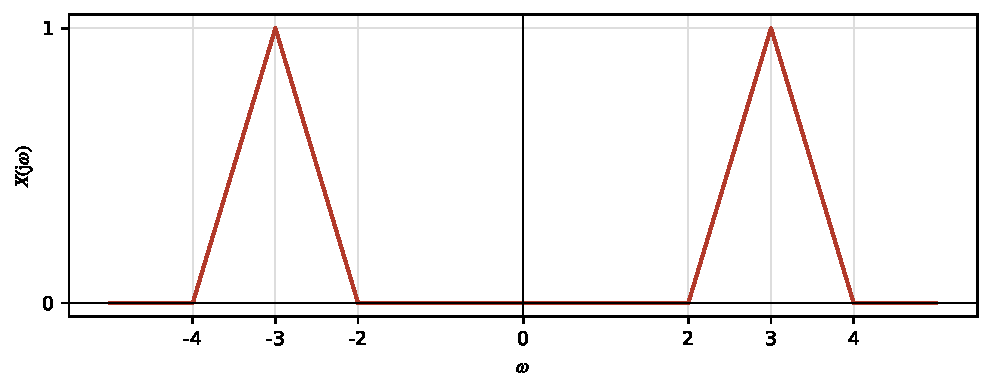
\includegraphics[width=0.72\textwidth]{06-ctft/examples/two-triangle-given.pdf}
    \caption{例题 \ref{ex:ctft-two-triangle-spectra} 的频谱。}
    \label{fig:ex-ctft-two-triangle-given}
  \end{figure}
\end{workedexample}

\begin{solution}
  先求中心在原点的单位三角频谱
  $G(\iu\omega)=\max(1-|\omega|,0)$ 的逆变换。
  将三角形拆成两个宽度为 $1$ 的矩形频谱的卷积。取
  $R_1(\omega)=2\pi\mathbf 1_{|\omega|<1/2}$、
  $R_2(\omega)=\mathbf 1_{|\omega|<1/2}$，对应的时域信号为
  \[
    \frac{2\sin(t/2)}{t}\fourierpair R_1(\omega),
    \qquad
    \frac{\sin(t/2)}{\pi t}\fourierpair R_2(\omega).
  \]
  频域滑动时，$R_1(\nu)$ 固定在 $[-1/2,1/2]$，$R_2(\omega-\nu)$ 移到 $[\omega-1/2,\omega+1/2]$。重叠区间内乘积为 $2\pi$，再乘频域卷积系数 $1/(2\pi)$：
  \[
    \frac1{2\pi}(R_1\conv R_2)(\omega)=
    \begin{cases}
      \displaystyle\frac1{2\pi}\int_{-1/2}^{\omega+1/2}2\pi\dd\nu
         =1+\omega,&-1\le\omega\le0,\\[5pt]
      \displaystyle\frac1{2\pi}\int_{\omega-1/2}^{1/2}2\pi\dd\nu
         =1-\omega,&0<\omega\le1,\\
      0,&|\omega|>1.
    \end{cases}
  \]
  这就是 $G$，所以
  \[
    g(t)=\frac{2\sin(t/2)}{t}\,
          \frac{\sin(t/2)}{\pi t}
        =\frac{2\sin^2(t/2)}{\pi t^2}.
  \]
  将频谱分别平移到 $\pm3$ 并相加，对应时域乘以两项复指数之和：
  \[
    x(t)=g(t)\bigl(\e^{\iu3t}+\e^{-\iu3t}\bigr)
        =\frac{4\sin^2(t/2)\cos(3t)}{\pi t^2}.
  \]
  $t=0$ 处按极限取值 $x(0)=1/\pi$，也等于频谱总面积除以 $2\pi$。时域波形见\cref{fig:ex-ctft-two-triangle-answer}。
  \begin{figure}[H]
    \centering
    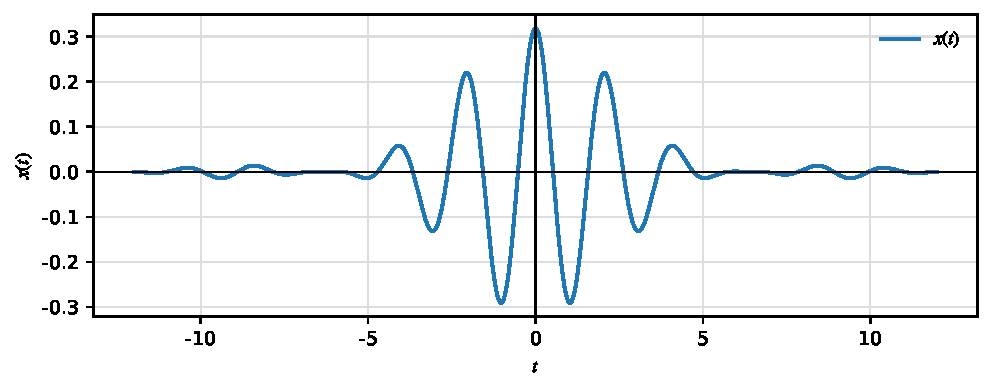
\includegraphics[width=0.72\textwidth]{06-ctft/examples/two-triangle-answer.pdf}
    \caption{例题 \ref{ex:ctft-two-triangle-spectra} 恢复出的信号。}
    \label{fig:ex-ctft-two-triangle-answer}
  \end{figure}
\end{solution}

\begin{technique}
  \hl{先把频谱移回原点并识别形状}，再处理频移。三角频谱写成两个矩形的卷积后，逆变换就是\red{两个 sinc 信号相乘}；对称的\red{正、负频移最终合成余弦}。
\end{technique}

\begin{workedexample}[用能量归一化确定波形]
  \label{ex:ctft-parseval-normalize}
  设 $A>0$，且 $X(\iu\omega)$ 满足
  \[
    \IFT\bigl[(2+\iu\omega)X(\iu\omega)\bigr]
    =A\e^{-t}\stepfun(t),
  \]
  \[
    \frac{1}{2\pi}\int_{-\infty}^{\infty}|X(\iu\omega)|^2\dd\omega=1.
  \]
  求 $x(t)$。
\end{workedexample}

\begin{solution}
  第一式说明 $(2+\iu\omega)X(\iu\omega)$ 是 $A\e^{-t}\stepfun(t)$ 的变换，
  \[
    (2+\iu\omega)X(\iu\omega)=\frac{A}{1+\iu\omega}.
  \]
  分解
  \[
    X(\iu\omega)
    =\frac{A}{(1+\iu\omega)(2+\iu\omega)}
    =A\left(\frac{1}{1+\iu\omega}-\frac{1}{2+\iu\omega}\right),
  \]
  逐项逆变换，
  \[
    x(t)=A(\e^{-t}-\e^{-2t})\stepfun(t).
  \]
  第二式就是 $\int_{-\infty}^{\infty}|x(t)|^2\dd t=1$。计算
  \begin{align*}
    \int_0^{\infty}(\e^{-t}-\e^{-2t})^2\dd t
    &=\int_0^{\infty}(\e^{-2t}-2\e^{-3t}+\e^{-4t})\dd t\\
    &=\frac12-\frac23+\frac14=\frac{1}{12}.
  \end{align*}
  于是 $A^2/12=1$。$A>0$，故 $A=2\sqrt{3}$，
  \begin{equation}
    x(t)=2\sqrt{3}\,(\e^{-t}-\e^{-2t})\stepfun(t).
    \label{eq:ex-ctft-parseval-answer}
  \end{equation}
  频域可以再核一次。$|X(\iu\omega)|^2=A^2/[(1+\omega^2)(4+\omega^2)]$，而
  \[
    \frac{1}{(1+\omega^2)(4+\omega^2)}
    =\frac13\left(\frac{1}{1+\omega^2}-\frac{1}{4+\omega^2}\right).
  \]
  从 $-\infty$ 到 $\infty$ 的积分等于 $\pi/6$，乘上 $A^2/(2\pi)$ 后仍是 $A^2/12$。波形见\cref{fig:ex-ctft-parseval-answer}。

  \begin{figure}[H]
    \centering
    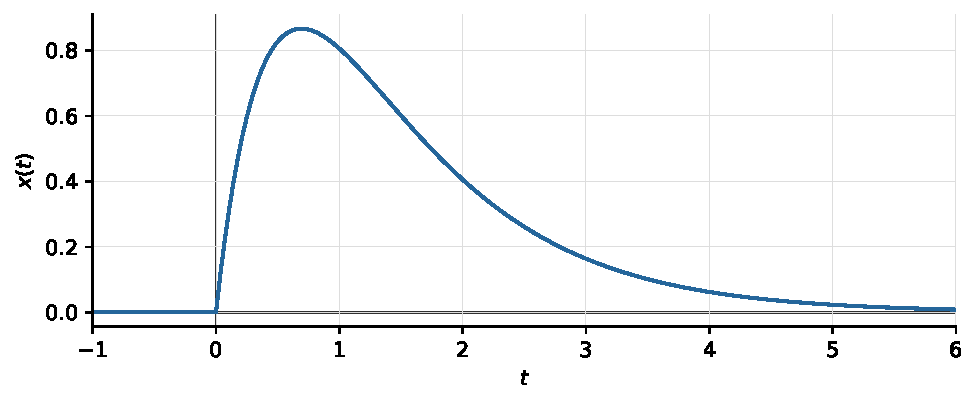
\includegraphics[width=0.72\textwidth]{06-ctft/examples/parseval-normalized-answer.pdf}
    \caption{例题 \ref{ex:ctft-parseval-normalize} 的信号。}
    \label{fig:ex-ctft-parseval-answer}
  \end{figure}
\end{solution}

\begin{technique}
  先利用乘以 $\iu\omega$ 或 $(a+\iu\omega)$ 的关系\hl{定出频谱形状}，\red{能量条件只负责一个正比例常数}。时域积分和帕塞瓦尔积分\red{应给出同一个常数}；两个结果不同时，\blue{先检查部分分式的符号}和 $1/(2\pi)$。
\end{technique}

\begin{workedexample}[用一个周期的变换求三角波系数]
  \label{ex:ctft-triangle-fs}
  设 $x(t)$ 以 $T>0$ 为周期，且为偶函数。在 $|t|<T/2$ 内
  \[
    x(t)=E\left(1-\frac{2|t|}{T}\right),
  \]
  峰值为 $E$，在 $t=\pm T/2$ 降到 $0$。求复系数 $A_k$，并写成余弦级数。波形见\cref{fig:ex-ctft-triangle-fs-given}。
  \begin{figure}[H]
    \centering
    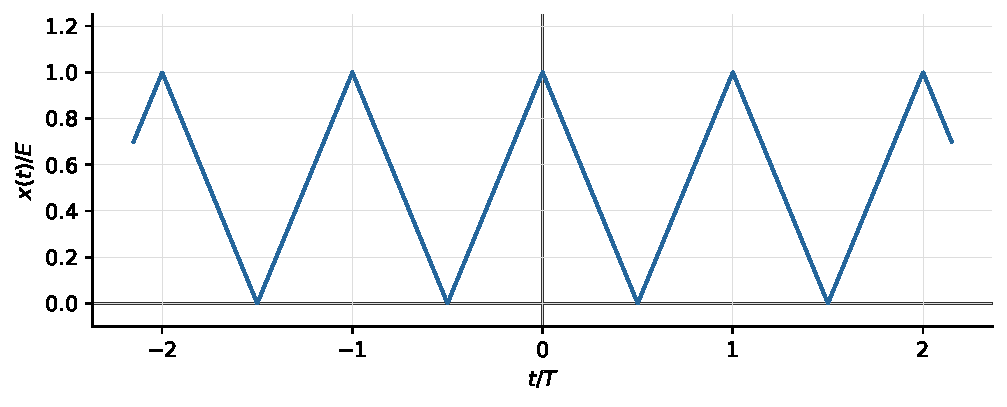
\includegraphics[width=0.72\textwidth]{06-ctft/examples/triangle-fs-given.pdf}
    \caption{例题 \ref{ex:ctft-triangle-fs} 的一个周期波形，横轴按 $T$ 归一化。}
    \label{fig:ex-ctft-triangle-fs-given}
  \end{figure}
\end{workedexample}

\begin{solution}
  取 $|t|<T/2$ 上的这一段，\blue{周期外置零}，记为 $x_1$。它是峰值 $E$、底宽 $T$ 的三角脉冲。对照\cref{eq:ctft-triangle-pair}，其中的底宽参数取 $T/2$，
  \[
    X_1(\iu\omega)=\frac{ET}{2}\Sa^2\!\left(\frac{\omega T}{4}\right).
  \]
  周期为 $T$ 时 $\omega_0=2\pi/T$。由\cref{eq:ctft-coefficient-from-transform}，
  \[
    A_k=\frac{1}{T}X_1(\iu k\omega_0)
    =\frac{E}{2}\Sa^2\!\left(\frac{k\pi}{2}\right).
  \]
  $\Sa(0)=1$，所以 $A_0=E/2$。$k\neq 0$ 时
  \[
    A_k=\frac{2E\sin^2(k\pi/2)}{\pi^2 k^2}.
  \]
  偶数 $k\neq 0$ 使 $\sin(k\pi/2)=0$，\red{对应系数为零}。信号为实偶函数，级数只含余弦：
  \begin{equation}
    x(t)=\frac{E}{2}
    +\sum_{m=0}^{\infty}
      \frac{4E}{\pi^2(2m+1)^2}
      \cos\bigl((2m+1)\omega_0 t\bigr).
    \label{eq:ex-ctft-triangle-fs-series}
  \end{equation}
  系数见\cref{fig:ex-ctft-triangle-fs-answer}。$k=\pm 1$ 时 $A_k/E=2/\pi^2$。

  \begin{figure}[H]
    \centering
    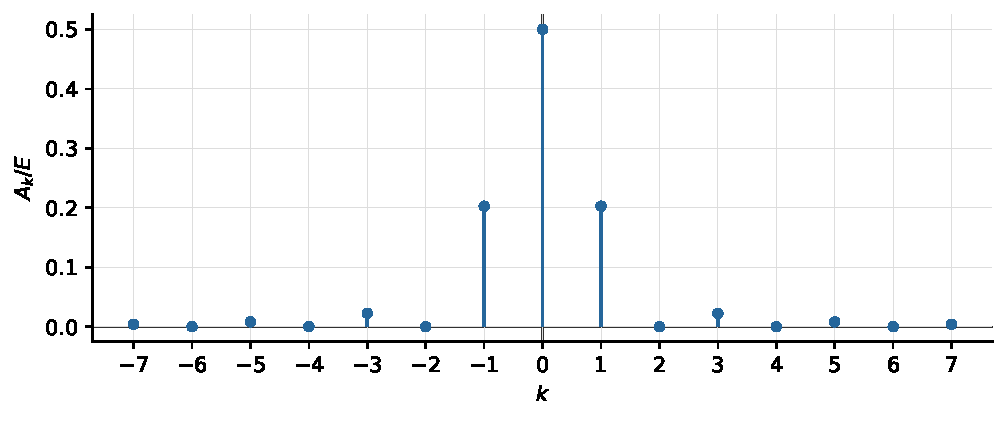
\includegraphics[width=0.72\textwidth]{06-ctft/examples/triangle-fs-answer.pdf}
    \caption{例题 \ref{ex:ctft-triangle-fs} 的复系数，纵轴按 $E$ 归一化。}
    \label{fig:ex-ctft-triangle-fs-answer}
  \end{figure}
\end{solution}

\begin{technique}
  \hl{先划出一个周期}并套已知的脉冲变换，再在 $k\omega_0$ 处取样、除以周期。\red{偶函数只有余弦项}。$\sin(k\pi/2)$ 在偶数 $k$ 为零，这些谐波可以\hl{在取样之前划掉}。
\end{technique}

\clearpage
\endgroup
